%
% File w266_paper.tex
%
%% Based on the style files for ACL 2020, which were
%% Based on the style files for ACL 2018, NAACL 2018/19, which were
%% Based on the style files for ACL-2015, with some improvements
%%  taken from the NAACL-2016 style
%% Based on the style files for ACL-2014, which were, in turn,
%% based on ACL-2013, ACL-2012, ACL-2011, ACL-2010, ACL-IJCNLP-2009,
%% EACL-2009, IJCNLP-2008...
%% Based on the style files for EACL 2006 by 
%%e.agirre@ehu.es or Sergi.Balari@uab.es
%% and that of ACL 08 by Joakim Nivre and Noah Smith

\documentclass[11pt,a4paper]{article}

\usepackage[hyperref]{w266_paper}
\usepackage{times}
\usepackage{latexsym}
\usepackage{graphicx}
\renewcommand{\UrlFont}{\ttfamily\small}

% This is not strictly necessary, and may be commented out,
% but it will improve the layout of the manuscript,
% and will typically save some space.
\usepackage{microtype}

%\aclfinalcopy % Uncomment this line for the final submission
%\def\aclpaperid{***} %  Enter the acl Paper ID here

%\setlength\titlebox{5cm}
% You can expand the titlebox if you need extra space
% to show all the authors. Please do not make the titlebox
% smaller than 5cm (the original size); we will check this
% in the camera-ready version and ask you to change it back.

\newcommand\BibTeX{B\textsc{ib}\TeX}

\title{QA System as an Answer Retrieval Problem}

\author{First Author \\
  Affiliation / Address line 1 \\
  Affiliation / Address line 2 \\
  Affiliation / Address line 3 \\
  \texttt{email@domain} \\\And
  Second Author \\
  Affiliation / Address line 1 \\
  Affiliation / Address line 2 \\
  Affiliation / Address line 3 \\
  \texttt{email@domain} \\}

\date{}

\begin{document}
\maketitle
\begin{abstract}
We plan to implement a Question Answering (QA) system for the financial industry. We plan to implement this using Transformer based models by restricting the scope to just the financial domain. We expect the input data to be a free-form text. We intend to explore new architectures involving pretrained models and fine tune them to retrieve the best answer from a large set of answers for a given question.

This research is not a first of its kind. We surveyed the literature and we found some very interesting related papers. Maia et.al [1] and Bithiah Yuan [4] used pairwise learning. While Maia et.al. did a comparative study that leveraged question context on pairwise learning, Bithiah Yuan focused on financial non-factoid answer selection and retrieved a  set of passage-level texts and selected the most relevant as the answer. Zhiyu Chen et.al. [3] performed numerical reasoning over financial data. Suman et. al. [5] provided a simplified approach and used SQuAD dataset to demonstrate their approach. Zhuang Liu et. al. [2] presented a domain specific language model pre-trained on large-scale financial corpora that enabled the capture of language knowledge and semantic information.

Our goal is to deliver a product that will help financial advisors to answer questions based on financial reports and/or disclosures. Often, there are inconsistencies and ambiguities in human interpretation. The outcome of our project will supplement FAQs automation, Chatbox, and dialog systems pertinent to the financial domain. 

\end{abstract}

\section{Introduction}

Add introduction section here.


\section{Related Work}
\label{sec:length}

Related work goes here.


\section{Our work}
We will try 3 approaches (1) Baseline Approach, (2) Two tower approach, and (3) Sentence Embedding.


\section{Baseline Approach}
Overview of our baseline QA pipeline. The inverted index retriever first returns the top k candidate answers. We will use the pretrained BERT mode with the financial corpus and by finetuning the pretrained BERT model to the target FiQA dataset. The output of the BERT model will pass the output to a softmax layer to assign a probability for each of the selected k answers and finally we will output the top n images within the selected k images.

\begin{figure}
  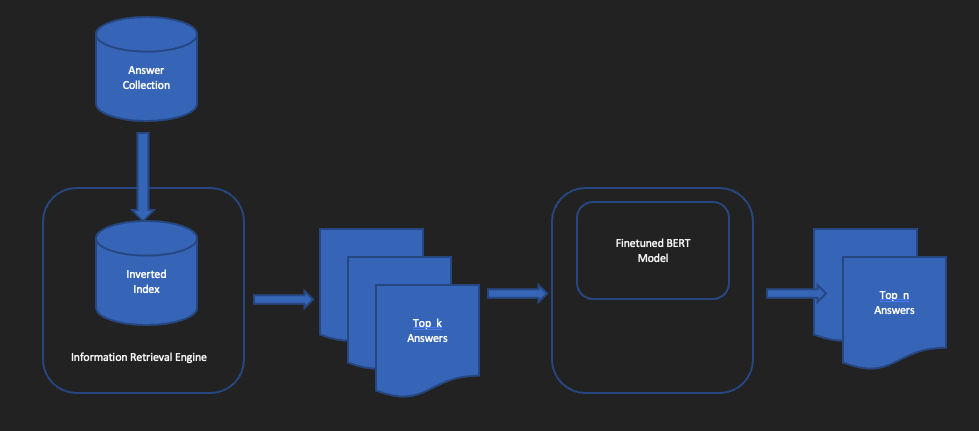
\includegraphics[width=\linewidth]{baseline.png}
  \caption{Baseline Model.}
  \label{fig:baseline model}
\end{figure}

\section{Two Tower Approach}
Papers that have been or will be submitted to other meetings or publications must indicate this at submission time in the START submission form, and must be withdrawn from the other venues if accepted by ACL 2020. Authors of papers accepted for presentation at ACL 2020 must notify the program chairs by the camera-ready deadline as to whether the paper will be presented. We will not accept for publication or presentation the papers that overlap significantly in content or results with papers that will be (or have been) published elsewhere.


\section{Approach using Sentence Embedding}
Papers that have been or will be submitted to other meetings or publications must indicate this at submission time in the START submission form, and must be withdrawn from the other venues if accepted by ACL 2020. Authors of papers accepted for presentation at ACL 2020 must notify the program chairs by the camera-ready deadline as to whether the paper will be presented. We will not accept for publication or presentation the papers that overlap significantly in content or results with papers that will be (or have been) published elsewhere.



\section{Metrics}
Papers that have been or will be submitted to other meetings or publications must indicate this at submission time in the START submission form, and must be withdrawn from the other venues if accepted by ACL 2020. Authors of papers accepted for presentation at ACL 2020 must notify the program chairs by the camera-ready deadline as to whether the paper will be presented. We will not accept for publication or presentation the papers that overlap significantly in content or results with papers that will be (or have been) published elsewhere.


\section{Results}
Papers that have been or will be submitted to other meetings or publications must indicate this at submission time in the START submission form, and must be withdrawn from the other venues if accepted by ACL 2020. Authors of papers accepted for presentation at ACL 2020 must notify the program chairs by the camera-ready deadline as to whether the paper will be presented. We will not accept for publication or presentation the papers that overlap significantly in content or results with papers that will be (or have been) published elsewhere.

\section{conclusion}
Papers that have been or will be submitted to other meetings or publications must indicate this at submission time in the START submission form, and must be withdrawn from the other venues if accepted by ACL 2020. Authors of papers accepted for presentation at ACL 2020 must notify the program chairs by the camera-ready deadline as to whether the paper will be presented. We will not accept for publication or presentation the papers that overlap significantly in content or results with papers that will be (or have been) published elsewhere.



\section*{Acknowledgments}

The acknowledgments should go immediately before the references. Do not number the acknowledgments section.
Do not include this section when submitting your paper for review.

\bibliography{anthology,acl2020}
\bibliographystyle{acl_natbib}

\appendix

\section{Appendices}
\label{sec:appendix}
Appendices are material that can be read, and include lemmas, formulas, proofs, and tables that are not critical to the reading and understanding of the paper. 
Appendices should be \textbf{uploaded as supplementary material} when submitting the paper for review.
Upon acceptance, the appendices come after the references, as shown here.


\end{document}
